\section{Valutazione prestazioni}

I test della versione OpenMP sono stati effettuati su una macchina equipaggiata
con una CPU Intel\textregistered\@ Core\texttrademark\@ i7--4710HQ quad core (8
thread) @ 2.50GHz ed una NVIDIA GeForce GTX 860M.

La valutazione delle prestazioni per la versione CUDA è stata invece effettuata
su una macchina equipaggiata con due processori Intel\textregistered\@
Xeon\textregistered\@ E5--2603 v4 hexa core @ 1.70GHz e tre GPU NVIDIA GeForce
GTX 1070.

Le tempistiche indicate sono state tutte ottenute mediante le funzioni di
libreria messe a disposizione dal docente. Per ulteriori informazioni si
consulti il codice sorgente.

\begin{figure}[!ht]
  \centering
  \begin{subfigure}[b]{0.49\linewidth}
  \centering
  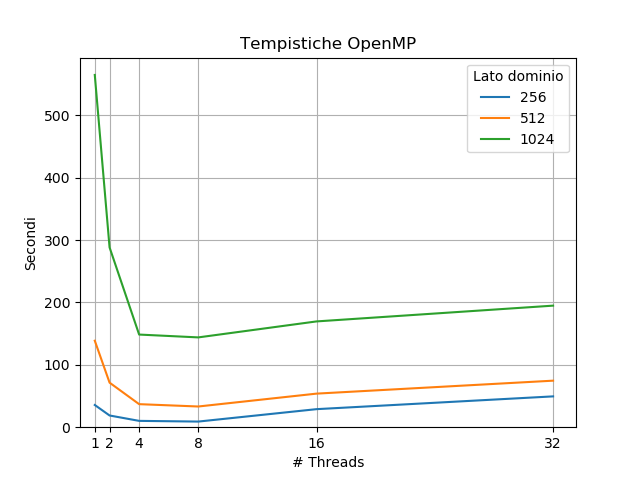
\includegraphics[scale=0.45]{./graphs/omp-timings.png}
  \caption{Comparazione tempistiche di esecuzione in
  OpenMP.}\label{fig:timingsomp1}
  \end{subfigure}
  \begin{subfigure}[b]{0.5\linewidth}
  \centering
  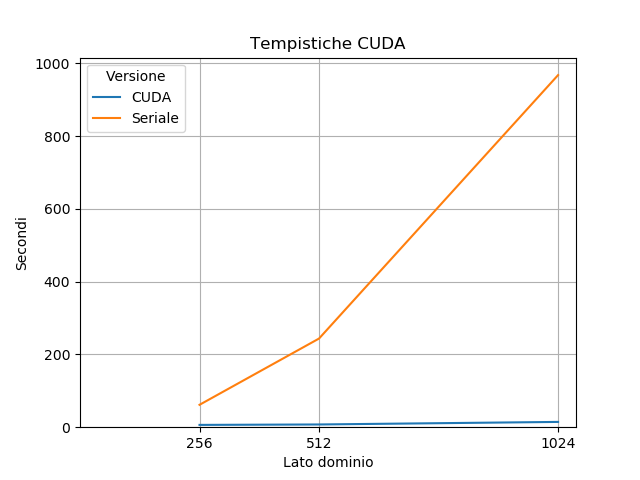
\includegraphics[scale=0.45]{./graphs/cuda-timings.png}
  \caption{Comparazione tempistiche di esecuzione in
  CUDA.}\label{fig:timingscuda1}
  \end{subfigure}
  \caption{Comparazione delle tempistiche di esecuzione dell'algoritmo.}\label{fig:timings}
\end{figure}

In figura \ref{fig:timingsomp1} è possibile notare che nell'esecuzione
dell'algoritmo implementato con parallelismo OpenMP il maggior guadagno si
registra nell'esecuzione in cui il dominio ha dimensione 1024 e che nelle
esecuzioni che usano più di 8 thread si ha un incremento di tempistiche.
Ciò è ancora una volta riconducibile ad un eccessivo carico di lavoro che lo
scheduler deve affrontare durante l'esecuzione del programma.

In figura \ref{fig:timingscuda1}, invece, è possibile osservare come la versione
CUDA vada ad abbattere drasticamente i tempi di esecuzione dell'algoritmo,
denotando un ingente guadagno prestazionale.

\subsection{Speedup}

Il calcolo dello speedup viene eseguito mediante la seguente formula:

\[
    S(p) = \frac{T_{serial}}{T_{parallel}(p)}
\]
in cui:
\begin{table}[ht]
\begin{tabular}{lll}
    p & : & \# processori/core\\
    T\textsubscript{serial}& : & tempo di esecuzione dell'algoritmo in versione
    seriale
    (T\textsubscript{serial}=T\textsubscript{parallel}(1))\\
    T\textsubscript{parallel}(\textit{p}) & : & tempo di esecuzione della
    versione parallela con \textit{p} processori/core
\end{tabular}
\end{table}

Poiché l'implementazione della soluzione contiene porzioni di codice non
parallelizzabili (si veda la funzione \texttt{setup}), dovremmo considerare
T\textsubscript{parallel}(\textit{p}) nel seguente modo:

\[ 
T_{parallel}(p) = \alpha \cdot T_{serial} +  \frac{(1 - \alpha) \cdot
T_{serial}}{p}
\]

in cui $\alpha$ è il fattore relativo alla porzione di codice non
parallelizzabile, calcolato come segue:

\[ 
\alpha = \frac{T_{serial}}{T_{serial} + T_{parallel}}.
\]

Tuttavia, come mostrato in tabella \ref{tab:alpha}, la porzione di codice
seriale (non parallelizzabile) impiega tempo trascurabile rispetto alla porzione
di codice parallelizzata, pertanto anche $\alpha$ assume valore trascurabile.

\begin{table}[ht]
\centering
\begin{tabular}{ccccc}
\toprule
 Lato dominio & Numero passi & T\textsubscript{seriale} (\textit{s}) &
 T\textsubscript{parallelo} (\textit{s})& $\alpha$ \\
 \midrule
    256 & \multirow{2}{*}{100000} & 0.00140063 & 14.2519 & 0.00009827 \\
    1024 & & 0.02356447 & 150.2037 & 0.00015686 \\
\bottomrule
\end{tabular}
\caption{Comparazione delle tempistiche per le porzioni seriale e parallele
dell'algoritmo.\label{tab:alpha}}
\end{table}

Per le siffatte osservazioni, considereremo
T\textsubscript{parallel}(\textit{p}) in tal modo:

\[
T_{parallel}(p) = \frac{T_{serial}}{p}.
\]

In figura \ref{fig:speedup1} è possibile osservare che lo speedup cresca fino a
8 thread, mantenendo di fatto la tendenza registrata nella misurazione delle
tempistiche.

\begin{figure}[!ht]
  \centering
  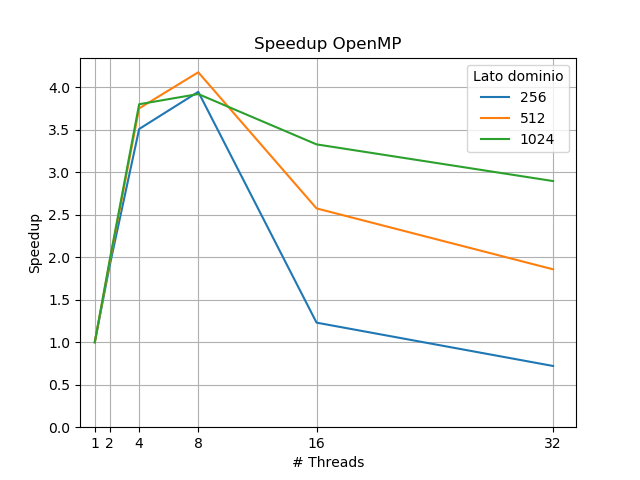
\includegraphics[scale=0.39]{./graphs/omp-speedup.png}
  \caption{Grafico dello speedup della versione OpenMP.}\label{fig:speedup1}
\end{figure}

\subsection{Scalabilità}

\subsubsection{Scalabilità forte}

La valutazione della scalabilità forte (\textit{strong scaling}), nonché i
risultati mostrati in figura \ref{fig:strong1} sono stati calcolati mediante
la seguente formula:

\[
    E(p) = \frac{S(p)}{p} = \frac{T_{serial}}{p \cdot T_{parallel}(p)}.
\]

\subsubsection{Scalabilità debole}

La valutazione della scalabilità debole (\textit{weak scaling}), nonché i
risultati mostrati in figura \ref{fig:weak1} sono stati calcolati mediante
la seguente formula:

\[
W(p) = \frac{T_{1}}{T_{p}}
\]

in cui:
\begin{table}[!ht]
\begin{tabular}{lll}
    p &: & \# processori/core\\
    T\textsubscript{1}&: & tempo di esecuzione di una unità di lavoro con un
    processore/core\\
    T\textsubscript{p}&: & tempo di esecuzione di \textit{p} unità di lavoro con
    \textit{p} processori/core
\end{tabular}
\end{table}

Poiché nella valutazione della scalabilità debole la dimensione del problema è
proporzionale al numero di processori/core utilizzati, il lato della matrice
utilizzata nell'algoritmo è stato calcolato come segue:

\[
side(p) = 256 \cdot \sqrt[3]{p}
\]

in cui 256 è la dimensione presa come lato di base.

\begin{figure}
  \centering
  \begin{subfigure}[b]{0.49\linewidth}
  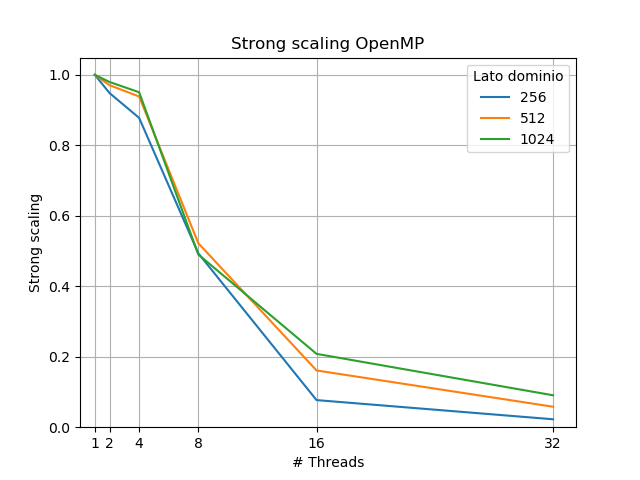
\includegraphics[scale=0.49]{./graphs/omp-strong.png}
  \caption{Grafico della scalabilità forte.}\label{fig:strong1}
  \end{subfigure}
  \begin{subfigure}[b]{0.5\linewidth}
  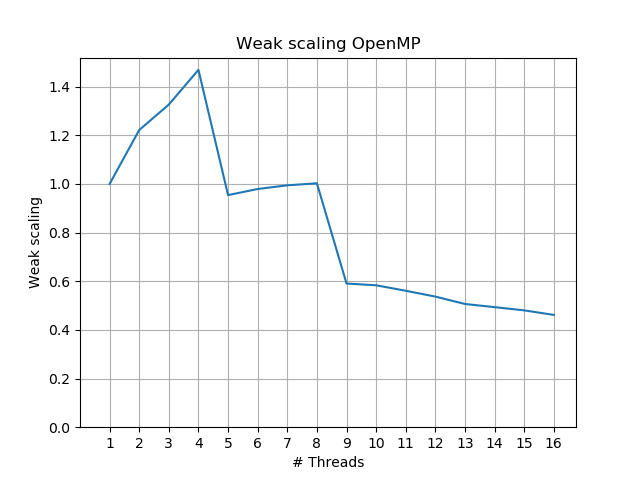
\includegraphics[scale=0.5]{./graphs/omp-weak.png}
  \caption{Grafico della scalabilità debole.}\label{fig:weak1}
  \end{subfigure}
  \caption{Grafici che rappresentano la scalabilità della versione OpenMP.}\label{fig:scaling}
\end{figure}
